% THIS IS SIGPROC-SP.TEX - VERSION 3.1
% WORKS WITH V3.2SP OF ACM_PROC_ARTICLE-SP.CLS
% APRIL 2009
%
% It is an example file showing how to use the 'acm_proc_article-sp.cls' V3.2SP
% LaTeX2e document class file for Conference Proceedings submissions.
% ----------------------------------------------------------------------------------------------------------------
% This .tex file (and associated .cls V3.2SP) *DOES NOT* produce:
%       1) The Permission Statement
%       2) The Conference (location) Info information
%       3) The Copyright Line with ACM data
%       4) Page numbering
% ---------------------------------------------------------------------------------------------------------------
% It is an example which *does* use the .bib file (from which the .bbl file
% is produced).
% REMEMBER HOWEVER: After having produced the .bbl file,
% and prior to final submission,
% you need to 'insert'  your .bbl file into your source .tex file so as to provide
% ONE 'self-contained' source file.
%
% Questions regarding SIGS should be sent to
% Adrienne Griscti ---> griscti@acm.org
%
% Questions/suggestions regarding the guidelines, .tex and .cls files, etc. to
% Gerald Murray ---> murray@hq.acm.org
%
% For tracking purposes - this is V3.1SP - APRIL 2009

\documentclass{acm_proc_article-sp}

\begin{document}

\title{Medipa: Visualizing Medical Scans in 3D on the Web}
%
% You need the command \numberofauthors to handle the 'placement
% and alignment' of the authors beneath the title.
%
% For aesthetic reasons, we recommend 'three authors at a time'
% i.e. three 'name/affiliation blocks' be placed beneath the title.
%
% NOTE: You are NOT restricted in how many 'rows' of
% "name/affiliations" may appear. We just ask that you restrict
% the number of 'columns' to three.
%
% Because of the available 'opening page real-estate'
% we ask you to refrain from putting more than six authors
% (two rows with three columns) beneath the article title.
% More than six makes the first-page appear very cluttered indeed.
%
% Use the \alignauthor commands to handle the names
% and affiliations for an 'aesthetic maximum' of six authors.
% Add names, affiliations, addresses for
% the seventh etc. author(s) as the argument for the
% \additionalauthors command.
% These 'additional authors' will be output/set for you
% without further effort on your part as the last section in
% the body of your article BEFORE References or any Appendices.

\numberofauthors{2} %  in this sample file, there are a *total*
% of EIGHT authors. SIX appear on the 'first-page' (for formatting
% reasons) and the remaining two appear in the \additionalauthors section.
%
\author{
% You can go ahead and credit any number of authors here,
% e.g. one 'row of three' or two rows (consisting of one row of three
% and a second row of one, two or three).
%
% The command \alignauthor (no curly braces needed) should
% precede each author name, affiliation/snail-mail address and
% e-mail address. Additionally, tag each line of
% affiliation/address with \affaddr, and tag the
% e-mail address with \email.
%
% 1st. author
\alignauthor
Juhee Bae\\
       \affaddr{North Carolina State University}\\
       \email{jbae3@ncsu.edu}
% 2nd. author
\alignauthor
Eric D. Helms\\
       \affaddr{North Carolina State University}\\
       \email{edhelms@ncsu.edu}
}
% There's nothing stopping you putting the seventh, eighth, etc.
% author on the opening page (as the 'third row') but we ask,
% for aesthetic reasons that you place these 'additional authors'
% in the \additional authors block, viz.
\date{12 December 2011}
% Just remember to make sure that the TOTAL number of authors
% is the number that will appear on the first page PLUS the
% number that will appear in the \additionalauthors section.

\maketitle
\begin{abstract}
We introduce Medipa, an open-source system to display medical images on the web that allows to share investigation from multiple medical representatives. It allows to upload the medical images, save configurations and comments, zoom-in and zoom-out, highlight, and slice the volume. The rendering algorithm is based on volume ray-tracing using shaders implemented in WebGL, javascript, and HTML5.
\end{abstract}

\terms{Volume rendering, WebGL, Medical images}
\section{Introduction}
The current state of the art for viewing medical image scans requires using a desktop application.  This means having the software installed on every computer a medical health practitioner wishes to view the scans on as well as ensuring that computer runs the required operating system and has the required packages installed. 

As web browser technology has evolved, access to the underlying GPU and APIs that follow the OpenGL standard have been added for doing complex 2D and 3D rendering.  This allows for the creation of complex applications using the browser as a platform that used to require a full desktop application.  The web provides a platform that is operating-system agnostic and allows users to use their favorite browser for interaction.  Further, by serving the content up from a central location, users can go anywhere in the world and still have access to viewing the scans.  This opens up a world where scans can be viewed by a variety of people and crowd-sourcing of ideas can be shared.

The rest of the paper is organized as follows: Section 2 provides a look at related works in the area of volume rendering, Section 3 talks about the concept, Section 4 covers details of the implementation, Section 5 discusses limitations and Section 6 finishes with conclusions and possible future work directions.


\section{Related Works}
The technique of volume rendering gained a lot of interest especially to investigate medical data. The process of volume rendering has several stages to produce the result image \cite{drebin:1988}. First, the input volume data set is converted to a set of material percentage volumes. Each element in the volume is called a voxel (volume element) which the value represents the percentage of the material in a region of space. After classifying the dataset, a linear ramp called a transfer function assigns the opacity and color values to every voxel in the volume. It allows viewing a certain part of the volume by selecting a certain range of opacity and color. Next, the volume is projected to the image plane by compositing the opacity and colors of the voxels. 

Previous researches attempted multiple methods to visualize volumes. Marching cubes \cite{lorensen:1987} provided an algorithm that creates polygonal representation of iso-surfaces from a three dimensional array of data. It uses a table of possible edge intersections of a cube which describes how a surface cuts the surface. For realism, it calculates the normalized gradient from the original data which helps to create the desired surface model. However, the drawback of the algorithm is the speed regarding to the great number of triangles and overhead by rotation. The amount of memory needed for the surface result is another problem. Also, there exists a hole problem which you see a hole of the result image when at least one cube face has an intersection point in each of its four edges.

Levoy\cite{levoy:1990} introduced an efficient way to use ray-tracing for volume rendering. It improves its performance by employing binary volumes of coherent regions and adaptively terminating ray-tracing at the user-selected opacity threshold. However, the method is not interactive.
For interactivity, splatting provided a way to perform volume rendering in parallel. It is a technique that splats every voxel to the viewing surface in back-to-front order as if throwing a snow ball to a wall \cite{westover:1991}. This method runs in parallel, thus reduces the rendering time, but produces respectively lower image qualities. 
Recently, interesting work on WebGL have been conducted with volume rendering \cite{anatomical:2011}. 


\section{Concept}
\subsection{Rendering algorithm}

Volume rendering displays 3D scalar field dataset to a 2D image. The two traditional ways are slice-based rendering and volume ray tracing. Our algorithm follows volume ray tracing that shoots rays through the volume and samples along the path by equal intervals. As the sampling points are advanced along the ray, it accumulates the opacity and RGB values of the sampling points. By the use of transfer function, it assigns the color and opacity values to each voxel in the volume and shows the corresponding emission and absorption of light for the sample point. The transfer function enables to observe a specific part of the volume given the range of the density value in the dataset. We allowed easier interaction with the visual controls to manipulate the range of the dataset as well as the color and opacity values on the client side. 
The advantages of ray tracing are optimization from empty space skipping, independence of the projection view, and easiness of development. In order to improve performance, the algorithm renders the position of front and back facing triangles to the textures instead of calculating the intersection between the ray and the bounding box around the volume. The front face texture provides the start position of the ray and the result of subtracting from back to front face texture provides the direction of the ray. Then, starting from the start position of each ray, the algorithm accumulates the color and opacity value of the sampling point in front-to-back direction in parallel. In addition, the process is optimized to stop earlier when the accumulated opacity reaches to the maximum value (i.e.,1.0) or when the advance of ray tracing reached the length of the ray. It is possible by the back face texture which contains the end position of the ray for each pixel. The code is shown below.



$vec3 raystart = v_PosLocal; \\
vec2 texcoords = (v_Position.xy / v_Position.w + vec2(1.0, 1.0)) / 2.0; \\
vec3 rayend = texture2D(backpos_tex, texcoords).xyz; \\
vec3 raydir = rayend - raystart; \\
vec3 deltadir = normalize(raydir) * stepsize; \\
float len = length(raydir); \\
float deltadirlen = length(deltadir); \\
vec3 raypos = raystart + steps * interstep * deltadir; \\
float lengthsum = steps * interstep * deltadirlen; \\
vec4 colorsum = mix(vec4(0.0, 0.0, 0.0, 0.0), texture2D\\(intermediate_tex, texcoords), clamp(interstep, 0.0, 1.0)); \\
vec4 colorsample; \\
\\
for (float i = 0.0; i < steps; i += 1.0) \{ \\
	if (lengthsum >= len || colorsum.a >= 1.0) break; \\
	colorsample = tex3D(raypos); \\
	colorsample.a *= stepsize * opacity; \\
	colorsum.rgb += colorsample.rgb * colorsample.a * (1.0 - colorsum.a); \\
	colorsum.a += colorsample.a * (1.0 - colorsum.a); \\
	raypos += deltadir; \\
	lengthsum += deltadirlen; \\
\} \\
\\
gl_FragColor = mix(colorsum, vec4(colorsum.rgb * \\clamp(colorsum.a, 0.0, 1.0) *  brightness, 1.0), finalstep); $\\


We used WebGL, javascript, and HTML5 for implementing volume ray tracing. We also refered to previous work performed on volume rendering with WebGL \cite{anatomical:2011}. The details are described in the following section about the system. 

\begin{figure*}[htb]
\begin{center}
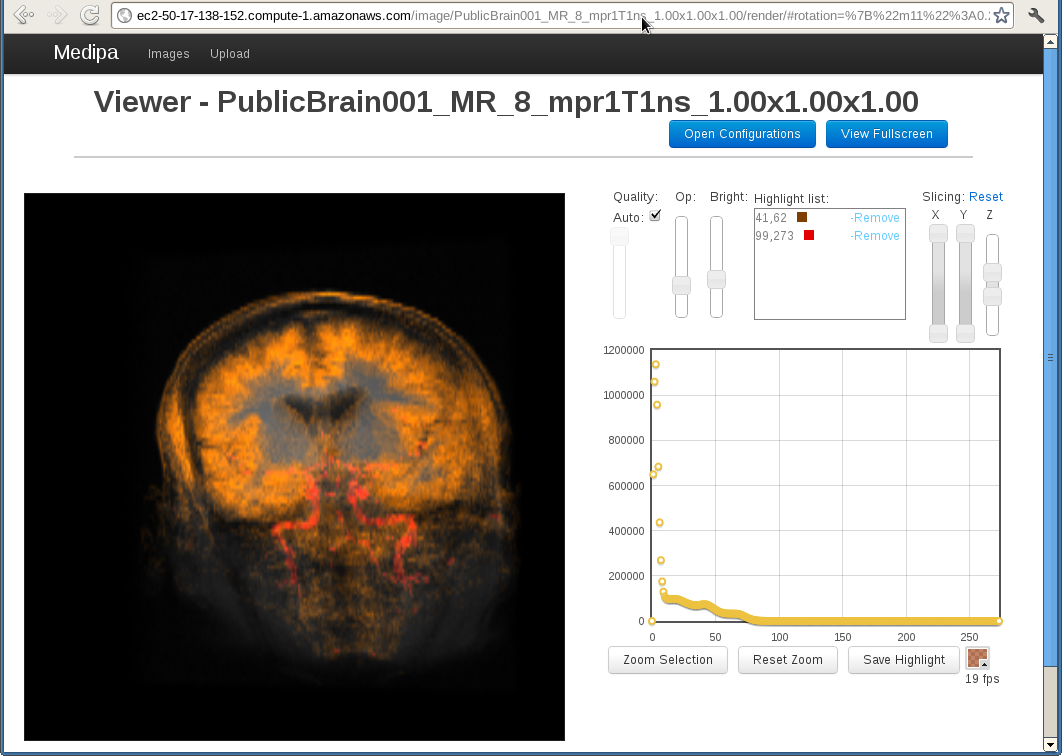
\includegraphics[scale=0.45]{head.png}
\caption{\label{fig:head}Brain rendered with Medipa}
\end{center}
\end{figure*}


\begin{figure*}[htb]
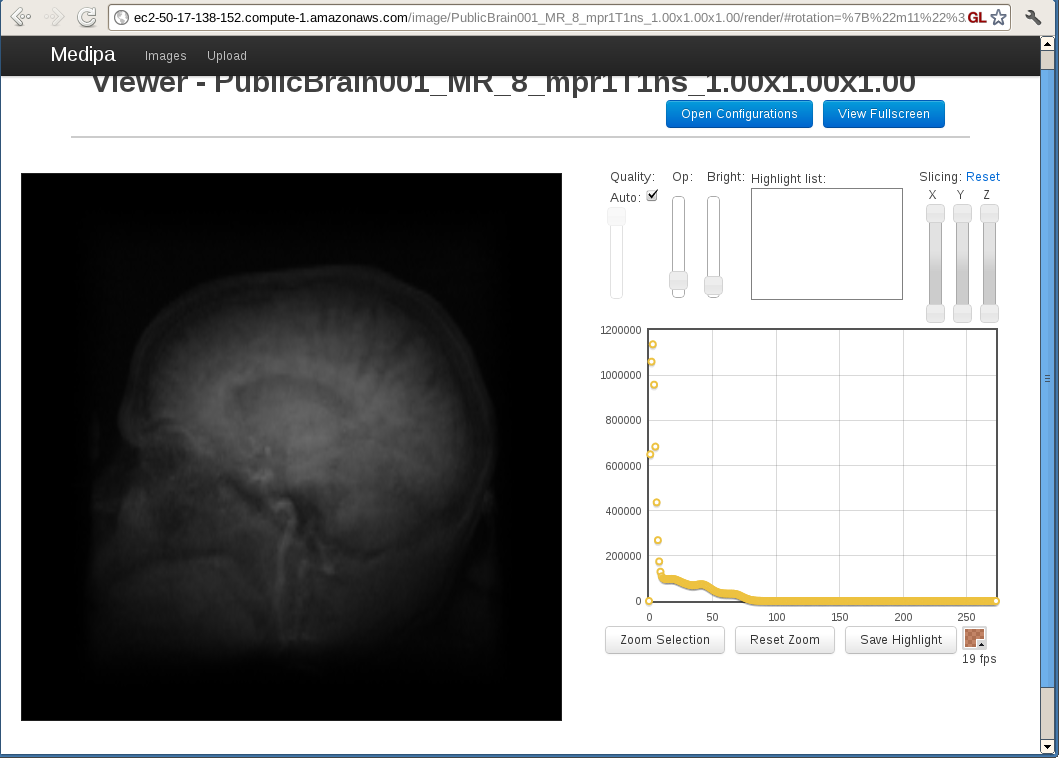
\includegraphics[scale=0.5]{clean_interface.png}
\label{Medipa System Architecture}
\end{figure*}

\section{Medipa}
The Medipa system was designed in order to allow users to upload or post URLs to medical image scans in their native formats, have them processed by an asynchronous task queue and provide an interactive rendering page for viewing the image scans as volume data.  Further, the rendering interaction provides users with tools to examine, modify and save user defined configurations of the rendered data.

\subsection{Architecture}
The underlying system was designed as a web-based Model-View-Controller (MVC) pattern with a data processing layer server side, asynchronous task queue and all rendering happening within the user's browser.  The architecture can be seen in Figure 2.

\begin{figure*}[htb]
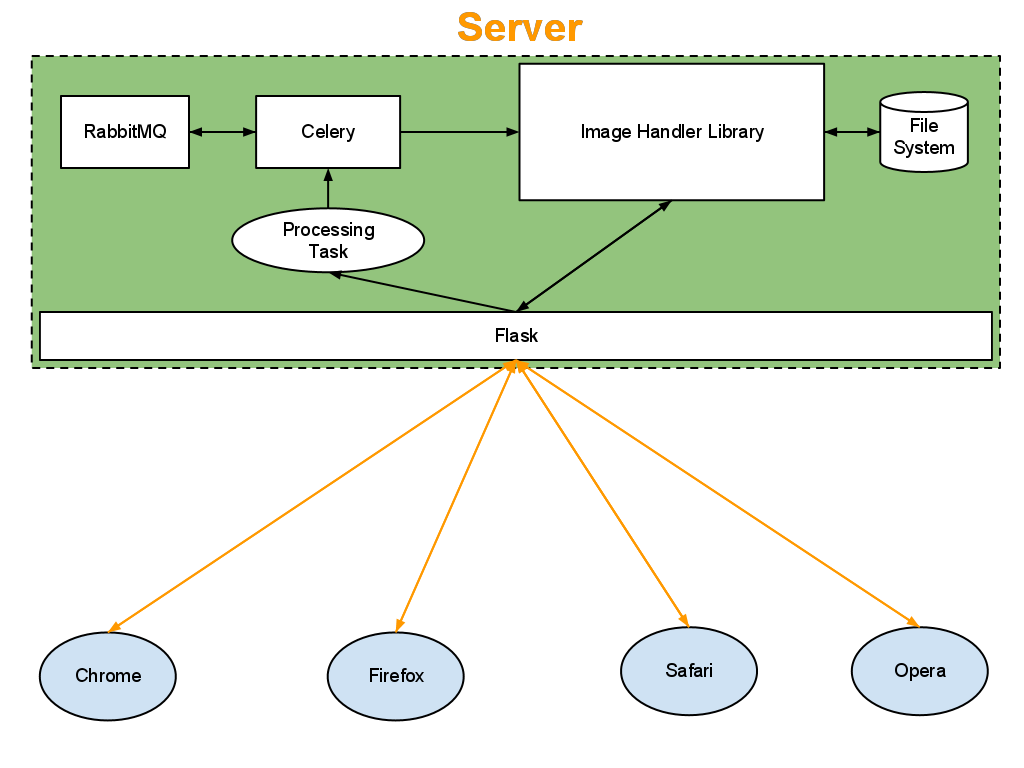
\includegraphics[scale=0.5]{architecture.png}
\label{Medipa System Architecture}
\end{figure*}

\subsubsection{Server}
	The server uses the Python micro web-framework Flask to create a set of urls and associate controllers for each.  Using the Jinja2 templating language, a series of templated HTML files that act as the views are associated with each controller action.  The model layer is handled by an image processing library that stores files to disk and uses a JSON formatted manifest file to store relevant data and references to files stored on disk.  Any call to retrieve or store data is processed through this library.
	The model layer is represented by a simple NoSQL JSON schema that is stored directly to the file system and processed by the code.

\subsubsection{Client Side}
We allow uploading custom image files (e.g., CT, MRI) or from urls. We provide interactive tools to zoom-in, zoom-out, highlight, and slice the volume. Zooming int and out the volume is enabled by manipulating the wheel control of a mouse. In order to select a specific range of the dataset, we display a histogram of the distribution of the density values of the dataset. The user can select a range by drag-and-drop interaction on the histogram and specify a point-of-interest of the volume data. The reason we use a histogram visualization is to see highly concentrated ranges that can be considered interesting regions of the data. It also ables to zoom in and out of the histogram by the x-axis to micro-select the range of the user's point of interest given the distributed values of the data. After the range selection, the user may choose a color to highlight the interested part on the image. The highlighted colors are listed and can be reordered by drag-and-drop interaction. In order to view inside the volume, the interface provides slider widgets to slice the volume on x, y, z axis, independently. In addition, since the tool is expected to share images, to be examined by multiple medical representatives, and commented when necessary, we provide a feature to save the current configuration and comments. The saved configurations can be loaded any time if a particular rendered image needs to be reviewd again. For performance adaptivity on different devices, we allow auto adjustment of image quality. The user can also control the opacity and brightness of the image when needed. The client is accessible online \footnote{ available at \url{http://ec2-50-17-138-152.compute-1.amazonaws.com/image/}}.

\subsection{Data Processing}

Most medical image scans come in a binary format that can not be directly ported to WebGL for rendering.  Given this limitation, a small data processing library was created taking advantage of SimpleITK.  SimpleITK is a library that can turn binary format medical scans into data representations that can be worked on within native code.  The layer would take in the binary medical scan format, process with SimpleITK and then turn the outputted pixel data array into a series of PNG's that represented each layer of the scan.  The subsequent PNG is saved down to the file system along with a JSON based file that contains metadata about the image.  This metadata included filenames, dimensions, configuration information and pixel histogram information.

Given that some systems may be limited in their graphical processing power, down 
sampling of the image resolution was added to the data processing layer.  Whenever an image is processed by the server, the data points are reduced 3 times and for each reduction a PNG is saved off and entry made into the manifest file.  The reductions occur by selecting an octet of the pixels and finding an average location and value.  This produces images that are 1/8, 1/64 and 1/512 the size and dimensions of the original image scan.

Down sampling the image provides two direct benefits that are related to the reliance on the client to handle rendering of the data.  The first benefit comes from being able to reduce the size of the image bundle being sent across the wire.  Low resolution images translate to small file sizes.  This in turn means that when the user first accesses the render page a small image can be sent quickly across for the user to start viewing and interacting automatically.  As time progresses, the system can fetch higher resolution images and swap them in behind the scenes for the user to allow continued interaction without interruption.  

The second benefit comes from the variability in client computer graphics processing power.  Attempting to render high resolution images on an under powered machine can not only place the application into an unusable state but also render the entire client machine unusable by the user as the CPU and GPU attempt to handle the large resolution.  Thus, having lower resolution images helps to allow users with under powered machines to still interact with the system.  Further, the client code monitors the frames-per-second (FPS) as each data resolution is brought in and will halt the quality increases if the code determines that the system would enter an unusable state.

\begin{figure*}[htb]
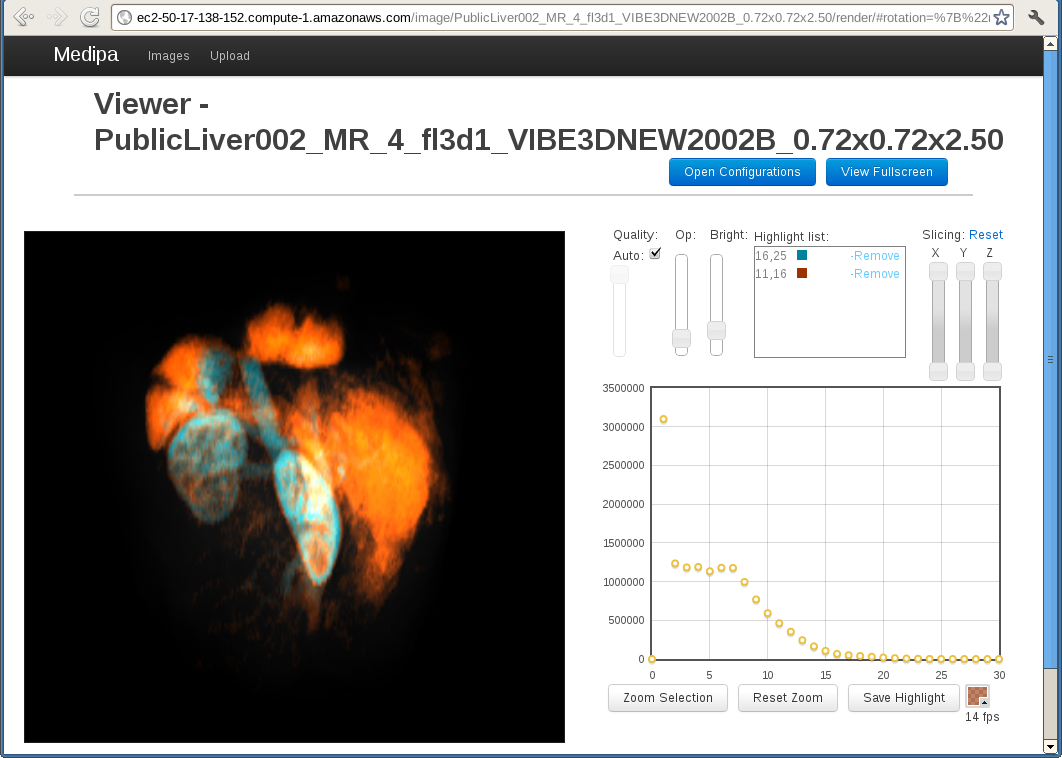
\includegraphics[scale=0.5]{kidneys.png}
\label{Medipa System Architecture}
\end{figure*}

\section{Limitations}
Given that typical medical image scans consist of multiple high resolution slices, processing of the image data is resource intensive task.  While the system takes measures to balance the performance on the users browser, the server side processing still requires a particular level of system performance in order to process images and serve data up in a reasonably performant amount of time.

A limitation of the worked perform thus far is the lack of direct input from medical professionals using the system.  Medical professionals would be the ultimate authority in providing feedback on both the interaction mechanisms as well as the extra visualization information such as pixel histogram designed to enhance the visual.		

\section{Future Work} 
The current model layer uses a JSON file saved to and accessed directly to the file system to store properties for each uploaded image.  This method does not provide the most robust solution for persistent data or any benefits of modern database systems.  Future work could include a transition to storing data within a NoSQL database.

The current system allows for users to define and store configurations of visualization properties for a given image file and include a comment related to the configuration.  Future work could include a more social or crowd-sourced annotation set by allowing a comment thread to be attached to each configuration.  Further, users could be allowed to create derivative visual configurations in response to an original in order to display what they find to other users.

\section{Conclusions}

The Medipa system aims to provide an interactive visualization of 3D volume rendering of medical image scans using a browser based solution with WebGL.



%
% The following two commands are all you need in the
% initial runs of your .tex file to
% produce the bibliography for the citations in your paper.
\bibliographystyle{abbrv}
\bibliography{sigproc}  % sigproc.bib is the name of the Bibliography in this case
% You must have a proper ".bib" file
%  and remember to run:
% latex bibtex latex latex
% to resolve all references
%
% ACM needs 'a single self-contained file'!
%
%APPENDICES are optional
%\balancecolumns
\appendix
%Appendix A

% This next section command marks the start of
% Appendix B, and does not continue the present hierarchy

\balancecolumns
% That's all folks!
\end{document}
